% !TEX TS-program = pdflatex
% !TEX encoding = UTF-8 Unicode

% This is a simple template for a LaTeX document using the "article" class.
% See "book", "report", "letter" for other types of document.

\documentclass[11pt]{article} % use larger type; default would be 10pt

\usepackage[utf8]{inputenc} % set input encoding (not needed with XeLaTeX)

%%% Examples of Article customizations
% These packages are optional, depending whether you want the features they provide.
% See the LaTeX Companion or other references for full information.

%%% PAGE DIMENSIONS
\usepackage{geometry} % to change the page dimensions
\geometry{a4paper} % or letterpaper (US) or a5paper or....
% \geometry{margin=2in} % for example, change the margins to 2 inches all round
% \geometry{landscape} % set up the page for landscape
%   read geometry.pdf for detailed page layout information

\usepackage{graphicx} % support the \includegraphics command and options

% \usepackage[parfill]{parskip} % Activate to begin paragraphs with an empty line rather than an indent

%%% PACKAGES
\usepackage{booktabs} % for much better looking tables
\usepackage{array} % for better arrays (eg matrices) in maths
\usepackage{paralist} % very flexible & customisable lists (eg. enumerate/itemize, etc.)
\usepackage{verbatim} % adds environment for commenting out blocks of text & for better verbatim
\usepackage{subfig} % make it possible to include more than one captioned figure/table in a single float
\usepackage{graphicx} % images
% \graphicspath{ {C:/Users/mingf/Desktop/git/twitter-sentiment-analysis/images} }
% These packages are all incorporated in the memoir class to one degree or another...

%%% HEADERS & FOOTERS
\usepackage{fancyhdr} % This should be set AFTER setting up the page geometry
\pagestyle{fancy} % options: empty , plain , fancy
\renewcommand{\headrulewidth}{0pt} % customise the layout...
\lhead{}\chead{}\rhead{}
\lfoot{}\cfoot{\thepage}\rfoot{}

%%% SECTION TITLE APPEARANCE
\usepackage{sectsty}
\allsectionsfont{\sffamily\mdseries\upshape} % (See the fntguide.pdf for font help)
% (This matches ConTeXt defaults)

%%% ToC (table of contents) APPEARANCE
\usepackage[nottoc,notlof,notlot]{tocbibind} % Put the bibliography in the ToC
\usepackage[titles,subfigure]{tocloft} % Alter the style of the Table of Contents
\renewcommand{\cftsecfont}{\rmfamily\mdseries\upshape}
\renewcommand{\cftsecpagefont}{\rmfamily\mdseries\upshape} % No bold!

%%% END Article customizations

%%% The "real" document content comes below...

\title{A Linguistic Analysis of Twitter Tweets for Donald J. Trump}
\author{Ming Fong\\
University of California, Berkeley\\
Linguistics 55AC}
%\date{} % Activate to display a given date or no date (if empty),
         % otherwise the current date is printed 

\begin{document}
\maketitle

\section{Introduction}

In the past decade, politicians, business leaders, and celebrities have increasingly turned to social media to reach a wider audience.
Of the many platforms available, Twitter has become one of the most popular social media outlets for those looking to reach a large follower base.
Among Twitter's most influential users is President Donald J. Trump.
President Trump's use of Twitter has ranged from attacks against political opponents to updates on actions he has taken as President of the United States.
The President's frequent use of Twitter is unprecedented among American leaders and has led to criticism from opponents and praise from supporters.
In this paper, we will explore linguistic trends of President Trump's Twitter posts with respect to the November 3, 2020 US Presidential election.
Specifically, we want to understand what it is that makes President Trump's use of Twitter so effective.

\section{Methodology}

We will collect Twitter Tweet text and the associated metadata from Tweets sent by from the account of Donald J. Trump (@realDonaldTrump).
Using that data, we can perform analyses on the various types of data we collect.

\subsection{Data Collection}

Our data will be directly sourced from Twitter using the Twitter Developer API.
We will read the tweets into a Pandas Dataframe containing the following columns:
$$["id"], ["date"], ["text"]$$
Due to limitations with the Twitter Developer API, our dataset is capped at the 3200 most recent tweets.
The timeframe of our data ranges from 14 September, 2020 to 11 December, 2020.
This allows us to establish a clear pattern both before and after the November 3, 2020 presidential election day.

\subsection{Data Analysis}

Before performing any analysis of the tweet text data, we must first clean the text.
Any non-alphanumeric characters and elements such as links are removed.
Additionally, all retweets are removed since their text were not written by President Trump.
An argument could be made to include retweets as they are constitutive of a user's usage pattern on Twitter.
However, because will be performing sentiment analysis, we will only keep text written by President Trump himself so that our metrics will be more reflective of his personal sentiment. 

Using the text of the tweets, we can assign a sentiment score to each tweet.
We do this using $textblob$, a Python module for text processing and sentiment analysis.
At a high level, $textblob$ assigns each word in a string of text a polarity value $p$ representing either positive sentiment $(0 < p < 1)$ or negative sentiment $(-1 < p < 0)$.
Modifier words such as "very", "greatly", or "extremely" and negation ("not") are taken into account and will scale the polarity or flip it respectively.
For each tweet, the calculated polarity scores for individual words are combined into a polarity score for the text of the entire tweet as a value between $-1$ and $1$.

We can also analyze metadata to discover trends or patterns in Twitter usage.
For example, looking at the timestamps of tweets sent yield some interesting visualizations.

\section{Analysis}

Our data collection and analysis was done using a Python Jupyter Notebook and the packages listed above.
The notebook and data files can be found below\footnote{Repository with analysis and data: https://github.com/evilpegasus/twitter-sentiment-analysis}.

\subsection{Data}

Our cleaned Dataframe with retweets and some characters removed looks like so

\begin{center}
    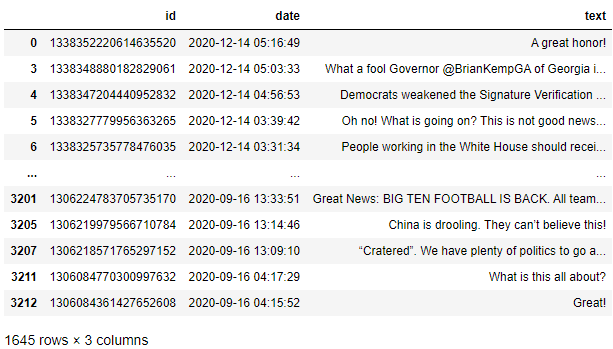
\includegraphics[width=0.57\paperwidth]{C:/Users/mingf/Desktop/git/twitter-sentiment-analysis/images/dataframe.PNG}
\end{center}

After removing retweets and links, we are left with 1645 rows of tweets. We are now ready to analyze the data.

\subsection{Linguistic Patterns}

From previous experience, we observed that President Trump has the tendency to repeat motifs and phrases in his speeches and addresses.
For example, his slogan "Make America Great Again" has been repeated at almost if not all rallies, and topics such as "China", the "trade war", and more recently "election fraud" are ubiquitous in Trump communications.
We suspect that the President will show a similar pattern in his tweets.
To test this theory, we can look at a word cloud of President Trump's tweet texts leading up to the November 3, 2020 election:

\begin{center}
    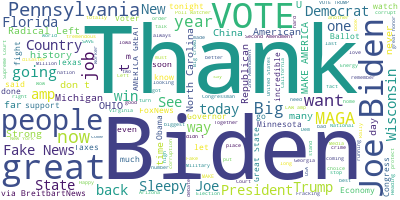
\includegraphics[width=0.6\paperwidth]{C:/Users/mingf/Desktop/git/twitter-sentiment-analysis/images/pre_wordcloud.png}
\end{center}

We can see that the most common word or phrase used was "Thank".
This suggests that Trump uses Twitter to target his supporters, as opposed to using Twitter as a media outlet for the press or news organizations.
Another word that appeared with high frequency was "Biden" and the associated "Joe Biden" and "Sleepy Joe".
The tweets mentioning Joe Biden were most likely attacks on him and his presidential campaign.
This is evidence of President Trump's very offensive style of campaigning where emphasis is placed on delegitimizing an opponent and their positions.
This aggressive and polarizing strategy is characteristic of not only his 2020 campaign, but of his entire presidency, and seems to have worked well considering his dedicated following.
The remaining words in the word cloud echo topics that Trump focused on during his campaign ("China", "job", "Economy") or states that he campaigned heavily in ("Pennsylvania", "Wisconsin", "Florida", "OHIO", etc.).

We can see that the tweets sent out before election day were very focused on his reelection campagin
However, after election day the words almost completely change
Below is the word cloud containing the most frequent words and phrases after November 3, 2020:

\begin{center}
    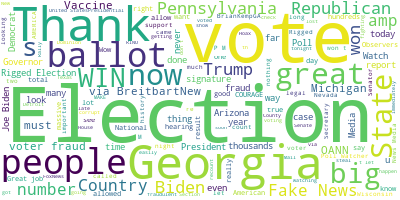
\includegraphics[width=0.6\paperwidth]{C:/Users/mingf/Desktop/git/twitter-sentiment-analysis/images/post_wordcloud.png}
\end{center}

Immediately, election-related words stand out as the most frequent ("Election", "vote", "ballot", "voter fraud").
Even after the election results, Trump has not given up on the presidency, and his Twitter usage shows that.
The states mentioned after election day have also shifted to the contested states that Biden took where Trump claims voter fraud ("Georgia", "Pennsylvania", "Michigan", "Arizona").
These post-election words are telling of Trump's focus on the election over a month after election day, which has overshadowed topics such as the coronavirus pandemic.

\subsection{Sentiment Analysis}

Using the techniques described in 2.2, we can analyze the general sentiment of tweets from President Trump.
Below is a graph of the mean sentiment per day:

\begin{center}
    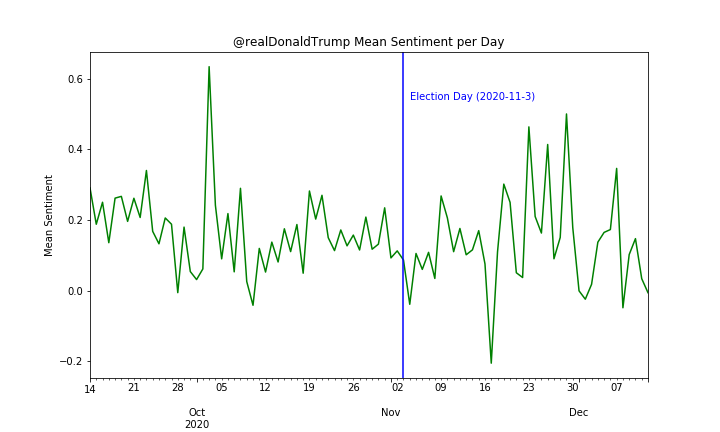
\includegraphics[width=0.6\paperwidth]{C:/Users/mingf/Desktop/git/twitter-sentiment-analysis/images/mean_sentiment_per_day.png}
\end{center}

It seems that President Trump's tweets generally have positive $(> 1)$ sentiment, with only a few days falling below a mean sentiment score of $0.0$.
However, there seems to be shift in general sentiment after election day, with post-election sentiment scores appearing lower and with higher variance than pre-election ones.
We can confirm this by calculating the percentage of days with positive sentiment and comparing the post and pre-election percentages.
Instead of $0.0$, we will use $0.25$ as the threshold for a positive day to minimize the impact of randomness or mislabeled sentiments.
The proportion of pre-election days with a mean sentiment score $> 0.25$ was $0.3007$ compared to $0.2643$ post-election.
Additionally, the mean sentiment score pre-election was $0.1497$ compared to $0.1216$ post-election.
Both these values confirm our suspicion that the sentiment scores dropped post-election.
Trump made fewer positive tweets after November 3, 2020 and the tweets were more negative when compared to pre-election data.

\subsection{Tweet Frequency}

From the timestamps of each tweet, we generate a plot of the number of tweets per day:

\begin{center}
    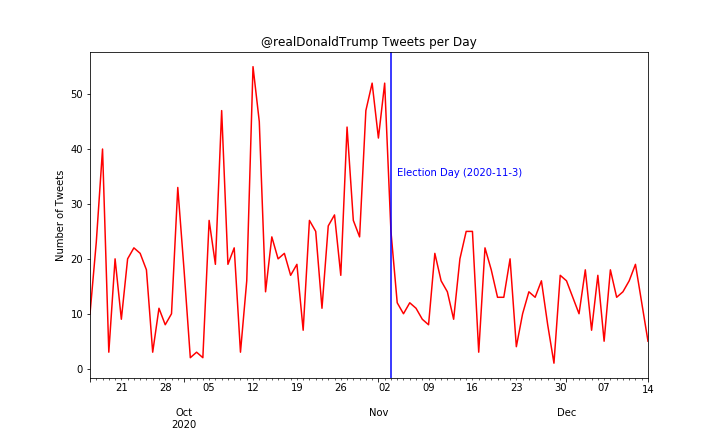
\includegraphics[width=0.6\paperwidth]{C:/Users/mingf/Desktop/git/twitter-sentiment-analysis/images/tweets_per_day.png}
\end{center}

Similar to the sentiment scores, we can visually observe a drop in the number of tweets per day following election day.
To confirm this, we can calculate the mean number of tweets per day pre and post election.
The mean number of tweets per day before election day was $22.354167$ compared to $13.619048$ post-election.
This is a very significant drop of nearly 40\% in tweet volume post-election.
We can safely conclude that after November 3rd, President Trump tweeted significantly less often than before election day.

\section{Conclusions}

From our analysis of various metrics of President Trump's twitter usage, it can concluded that Trump significantly changed the way he used twitter before and after the presidential election.
In the analysis of words and phrases most commonly used, we saw that President Trump shifted his focus from campagining to disputing the election results.
Additionally, sentiment analysis of the text of Trump's tweets showed a significantly less positive posts post-election when compared to pre-election data.
Finally, Trump's usage of the Twitter platform also fell post-election and he sent less tweets than before.

\subsection{Limitations}

The reseasrch and analysis done here have some technical limits that could be improved upon in the future.
Firstly, the dataset used was limited by the Twitter Developer API, which caps requests to the 3200 most recent tweets per user.
This limitation gave us data as far back as mid-September.
Ideally, we would have a more compelete set of data to work with.
Additionally, the $textblob$ package we used for sentiment analysis is quite naive in its calculations and may incorrectly score features like sarcasm.
Finally, because the November presidential election was a very recent event, we only have about a month of data following the event.
This may give rise to biases in the data that we are not aware of yet.

\section{References}

\begin{thebibliography}{}
    \bibitem{ouyang} 
    Yu Ouyang, and Richard W. Waterman. 
    \textit{Trump Tweets: A Text Sentiment Analysis. In: Trump, Twitter, and the American Democracy. The Evolving American Presidency}. 
    Palgrave Macmillan, Cham, 30 June 2020.
    \\\texttt{https://doi.org/10.1007/978-3-030-44242-2\_4}

    \bibitem{latexcompanion} 
    Efthymios Kouloumpis, Theresa Wilson, Johanna Moore. 
    \textit{Twitter Sentiment Analysis: The Good the Bad and the OMG!}. 
    Fifth International AAAI Conference on Weblogs and Social Media. 
    \\\texttt{https://citeseerx.ist.psu.edu/viewdoc/download?doi=10.1.1.682.5853\&rep=rep1\&type=pdf}
\end{thebibliography}

\end{document}
